%
%   Data preprocessing
%       - Data reading
%       - Checking missing value and data cleaning
%   
\section{Data preprocessing}



\subsection{Data reading}

\begin{code}{R}
pacman::p_load(
    rio,     # for dealing with basic import export
    ggplot2, # for dealing with plot formats
    zoo,      # for dealing with year quarter formats
    car     # for levent and shapiro
)
data <- import("./cpu-raw.csv") # rio::import
data <- data[, c("Status","Launch_Date",
         "Lithography","Recommended_Customer_Price",
         "nb_of_Cores","Processor_Base_Frequency",
                 "TDP","T")] 
\end{code}

The primary packages used in this process are:

\begin{itemize}
    \item \verb|rio| : for intuitive I/O code.
    With this package, import and export dataset is easier and safer. It could 
    also handle multiple file formats, so that we do not have to
    change the command each time we change the file format.

    \item \verb|zoo| : for year-quarter format.
    In our data, the \verb|Launch date| is in non-standard format, and difficult to be operated on. This package helps to transform
    into standard year-quarter format, and provides useful operations, such as plotting and taking difference on these formats.

    \item \verb|ggplot2| : is a famous plotting package for R language.

    \item \verb|car| : for the levent and shapiro for the assumption.
   % \item \verb|FSA| : for the post hoc test.
\end{itemize}

The rest of the code is just choosing the attributes that are useful for our purpose.

The original labels are very long and descriptive, we might not want that such level of details during coding. Therefore, the labels are suppressed
into small, compact abbreviations. Then, we export the code to \verb|cpu-clean.csv|.

\begin{code}{R}
names(data) <- c("status", "ldate", "litho", 
    "rprice", "ncore", "bfreq", "tdp", 
    "temp")

export("./cpu-clean.csv")
\end{code}

\begin{figure}[H]
    \centering
    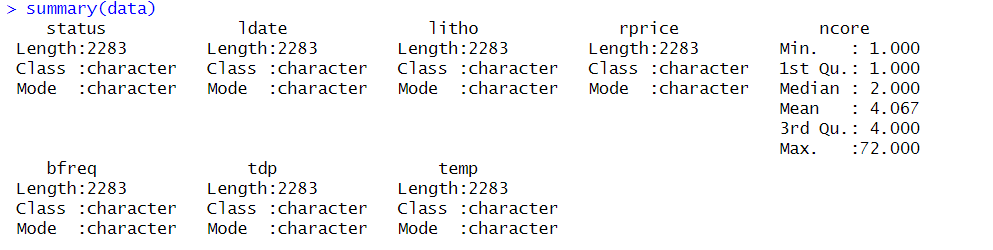
\includegraphics[max width=0.7\linewidth]{graphics/new_graphics/New data/summary-of-data-before.png}
    \caption{Summary of data before cleaning.}
\end{figure}

\subsection{Checking missing value and data cleaning}
\label{subsection:data_cleaning}

After choosing the approriate attributes, we now have the subset of the original raw dataset. 
However, since the values vary in types (such as string, non-standard year-quarter format and numeric-string),
we might want transform them into reproducible types, so that the analysis later on is easier, homogeneous and accurate.

Note that this cleaning process \textbf{does not} remove the \mintinline{R}{NA} values, unless necessary. The reason is that, 
in one instance, there might be important values that should not be eliminated. Under different scopes of study, we can not treat 
instances with \mintinline{R}{NA} as an invalid datum for all scopes. In later sections, when we focus on a specific pattern of the data, only by then
that the data will have a tailored \mintinline{R}{NA} cleaning, and we will not, by chance, loose any important instance.

This process took \verb|/rcode/cpu-short.csv| from the importing procedure above as an input, and produce \verb|/rcode/cpu-clean.csv| as
an output.

\begin{figure}[H]
    \centering
    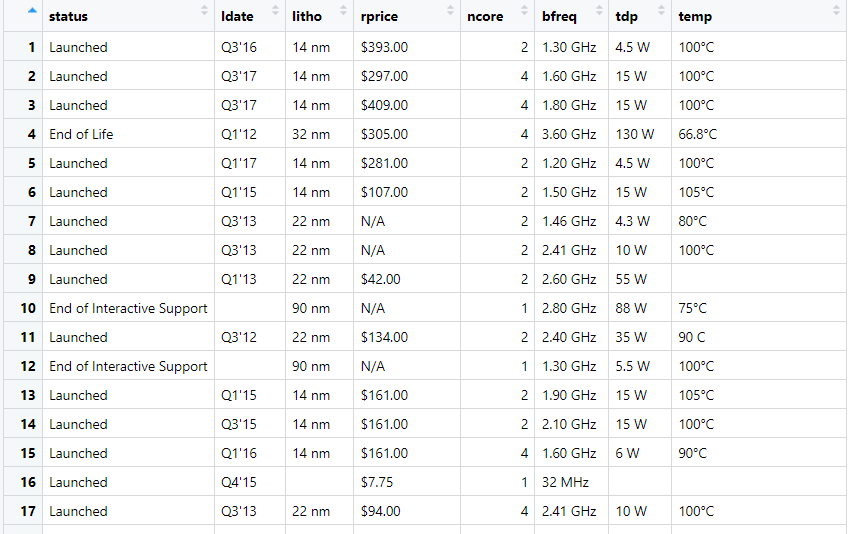
\includegraphics[max width=0.9\linewidth]{graphics/new_graphics/New data/Data-before.png}
    \caption{Data before cleaning.}
\end{figure}

\verb|market| and \verb|status| are left unchanged, since the values are straightforward. The remaining attributes (columns) are processed as followed:

\subsubsection*{Launch dates (ldate)}

\begin{code}{R}
data[,"ldate"] <- ( as.yearqtr(data[,"ldate"], format = "Q%q'%y"))
\end{code}

Our goal is to transform raw, non-standard year-quarter into \verb|zoo|'s standards. 
The function \mintinline{R}{as.yearqtr} takes a column and a format string as parameters. The format string is represented 
as: \mintinline{R}{"Q%q'%y"}, in which two flags \mintinline{R}{"%q"}, \mintinline{R}{"%y"} stands for quarter and year, respectively.
The format string hints the function to know the positions of quarter and year in our raw string.

\subsubsection*{Lithography (litho)}

\begin{code}{R}
data[,"litho"] <- as.numeric(gsub(" nm", "", data[,"litho"]))
\end{code}

Our goal is to cut out \verb|"nm"|, since every entry is recorded in nanometers anyway. In this code, \verb|gsub| substitutes 
the pattern \verb|" nm"| to \verb|""|. Notice that the pattern are regular expressions, and would be used intensively during 
this cleaning process.
% deprecated
\subsubsection*{Recommended Customer Price (rprice)}

\begin{code}{R}
data[,"rprice"] <- gsub("(^\\$(\\d)+.(\\d)+ - )", "", data[,"rprice"])
data$rprice <- ifelse(data$rprice == "N/A", NA, data$rprice)
data$rprice <- as.numeric(gsub('\\$|,', '', data$rprice))
\end{code}

Some \verb|rprice| values have ranges instead of sole numbers. We want to cut out uneccesary characters and only keep the largest price.
After that, we eliminate \verb|$| symbol from the string, as well as cast the string to numeric type.

\subsubsection*{Base frequency (bfreq)}

\begin{code}{R}
data[,"bfreq"] <- as.numeric(gsub("( GHz)|( MHz)", "", data[,"bfreq"]))
data<- data[!is.na(data$bfreq), ]
data$bfreq[data$bfreq > 10] <- data$bfreq[data$bfreq > 10]*0.001
\end{code}

Our goal is to cut out \verb|"GHz"| and \verb|"MHz"| from the string, and convert all \verb|"MHz"| values into \verb|"GHz"|. Heuristically,
we observed that any value greater than 10 must be \verb|MHz|, so we can transform every value like that will be multiply by 0.001 to get 
the according \verb|MHz| value.

\subsubsection*{Thermal design power (TDP)}
Same as for the \verb|litho| our goal is to simply also cut out W from the observation and change it to numeric type.

\begin{code}{R}
data[,"tdp"] <- as.numeric(gsub(" W", "", data[,"tdp"]))    
\end{code}

\subsubsection*{Temperature (temp)}

\begin{code}{R}
data[,"temp"] <- (gsub("[^0-9.\\-]+", ",", data[,"temp"]))
for (i in seq_along(data[["temp"]])) {
    temp_values <- strsplit(data[i, "temp"], ",") 
    temp_values <- unlist(lapply(temp_values, as.numeric))
    max_value <- max(temp_values, na.rm = TRUE)
    if (is.infinite(max_value)) {
        max_value <- NA
    }
    data[i, "temp"] <- max_value
}
export(data, "cpu-clean.csv")
\end{code}

Our goal is to only match the numeric values, then, take the maximum among those. The approach to processing the complicated strings in \verb|temp| is described as follows:
\begin{itemize}
    \item First, we attempt to match every decimal numbers possible, including the irrelevant number. The rest are replaced with commas \verb|","|.
    The result of this process will create a string of numbers separated by commas. By doing this, the numbers are well isolated for our purpose.

    \item Second, we split these numbers and form a vector of them. This can be done through \mintinline{R}{strsplit} function. Notice that our numbers
    are still in string format.

    \item Third, we cast all these strings to numeric and push them into a vector of values using \mintinline{R}{unlist} and \mintinline{R}{lapply}
    
    \item Fourth, we find the maximum among all these values. Invalid numbers will automatically become \(-\infty\), and will be further treated as \mintinline{R}{NA}.
    
    \item Notice that, we must loop through each row of the list to accomplish the above procedure.
\end{itemize}

Finally, the program produces \verb|cpu-clean.csv| as a cleaned data, ready for further exploitation in the later sections. In addition, \hyperlink{Listing 3}{\textit{\textcolor{blue}{Listing 3}}} and \hyperlink{Listing 4}{\textit{\textcolor{blue}{Listing 4}}} help us to identify the number of \mintinline{R}{NA} and \textbf{negative numbers}. Since there is no  \textbf{negative number} in our data, we skip the processing-with-negative-numbers process.

\begin{figure}[H]
    \centering
    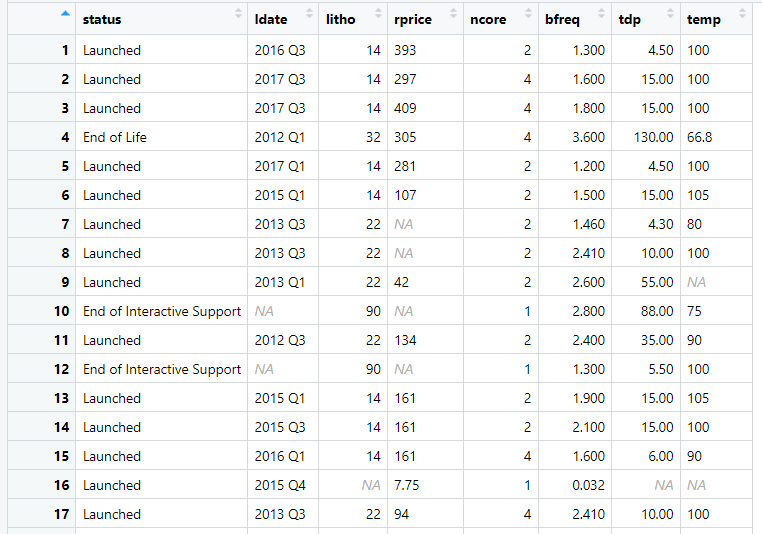
\includegraphics[max width=0.6\linewidth]{graphics/new_graphics/New data/Data-after.png}
    \caption{Data after cleaning.}
\end{figure}
\begin{code}{R}
    summary(data) ## Data summary after cleaning
    data$status<-as.factor(data$status)
    data$ldate<-as.factor(data$ldate)
    data$rprice<-as.factor(data$rprice)
    data$ncore<-as.factor(data$ncore)
    data$ncore<-as.factor(data$litho)
    ##Data summary by xtabs    
    xtabs(~status,data=data)
    xtabs(~ldate,data=data)
    xtabs(~litho,data=data)
    xtabs(~rprice,data=data)
    xtabs(~ncore,data=data)
    xtabs(~bfreq,data=data)
    xtabs(~tdp,data=data)
    xtabs(~temp,data=data)
\end{code}
\begin{figure}[H]
    \centering
    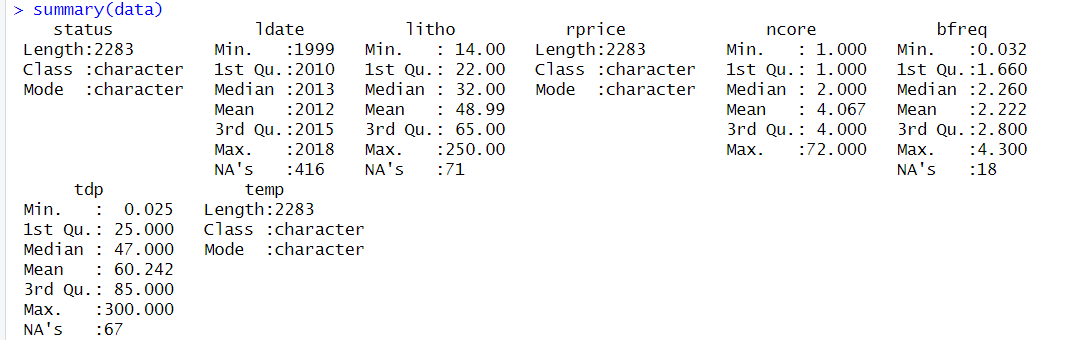
\includegraphics[max width=0.7\linewidth]{graphics/new_graphics/New data/summary-of-data-after.png}
    \caption{Data summary after cleaning.}
\end{figure}
\begin{figure}[!h]
\centering
    \begin{subfigure}[b]{0.49\textwidth}
        \centering
        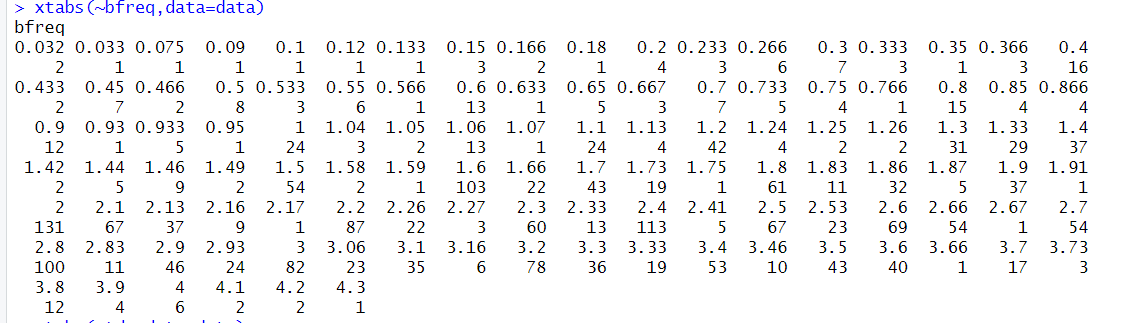
\includegraphics[width=\linewidth]{graphics/new_graphics/Xtabs/xtabs-bfreq.png}
        \caption{Summary of Base frequency.}
    \end{subfigure}
    \begin{subfigure}[b]{0.49\textwidth}
        \centering
        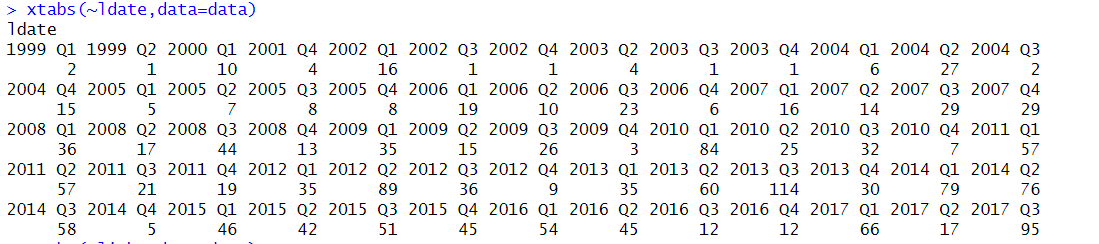
\includegraphics[width=\linewidth]{graphics/new_graphics/Xtabs/xtabs-ldate.png}
        \caption{Summary of Launch date.}
    \end{subfigure}
    \hfill
    \begin{subfigure}[b]{0.49\textwidth}
        \centering
        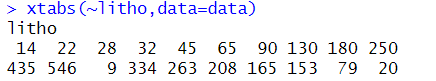
\includegraphics[width=\linewidth]{graphics/new_graphics/Xtabs/xtabs-litho.png}
        \caption{Summary of Lithography.}
    \end{subfigure}

    \begin{subfigure}[b]{0.49\textwidth}
        \centering
        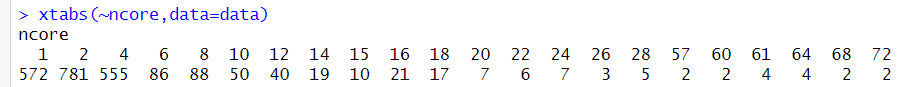
\includegraphics[width=\linewidth,height=0.4\linewidth]{graphics/new_graphics/Xtabs/xtabs-ncore.png}
        \caption{Summary of Number of Core.}
    \end{subfigure}
    \hfill
     \begin{subfigure}[b]{0.49\textwidth}
        \centering
        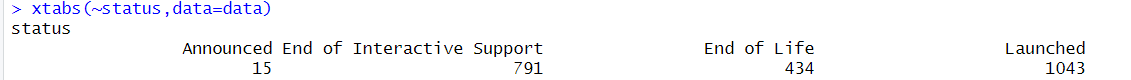
\includegraphics[width=\linewidth,height=0.4\linewidth]{graphics/new_graphics/Xtabs/xtabs-status.png}
        \caption{Summary of Status.}
    \end{subfigure}
    \begin{subfigure}[b]{0.49\textwidth}
        \centering
        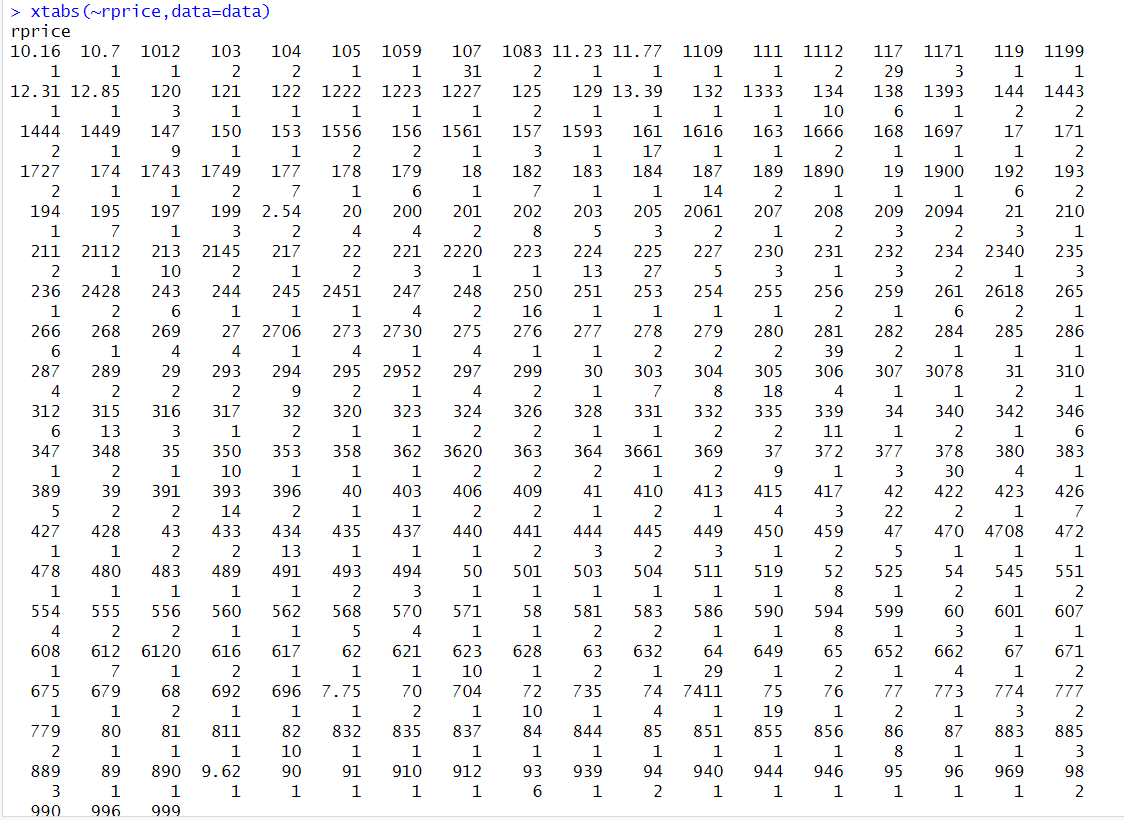
\includegraphics[width=\linewidth]{graphics/new_graphics/Xtabs/xtabs-rprice.png}
        \caption{Summary of Recommend Price.}
    \end{subfigure}
   \hfill
    \begin{subfigure}[b]{0.49\textwidth}
        \centering
        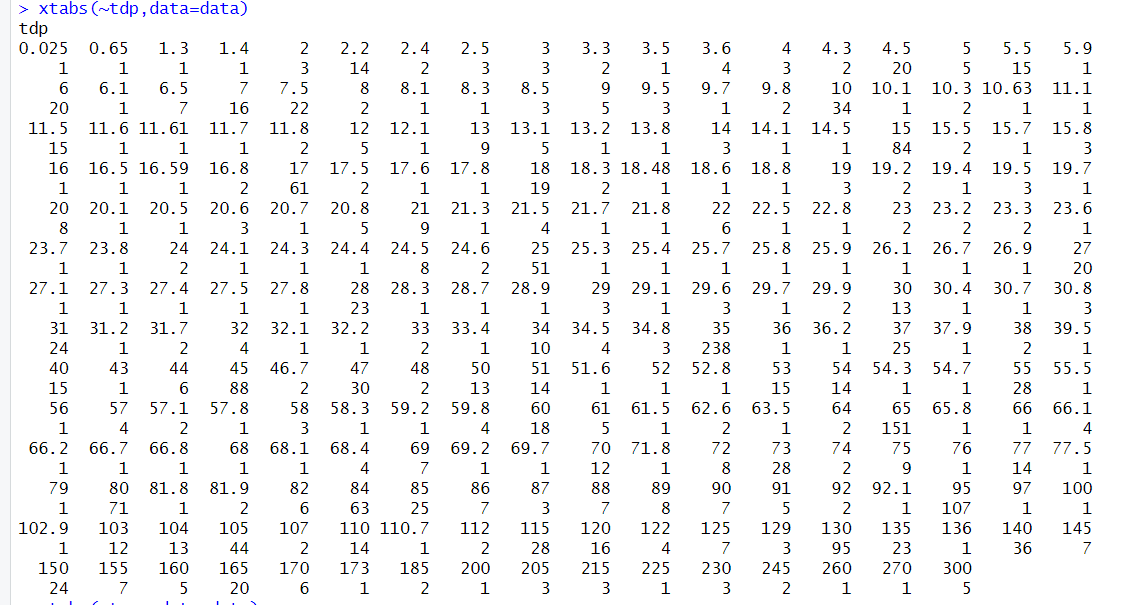
\includegraphics[width=\linewidth]{graphics/new_graphics/Xtabs/xtabs-tdp.png}
        \caption{Summary of Thermal design power.}
    \end{subfigure}
    \begin{subfigure}[b]{0.49\textwidth}
        \centering
        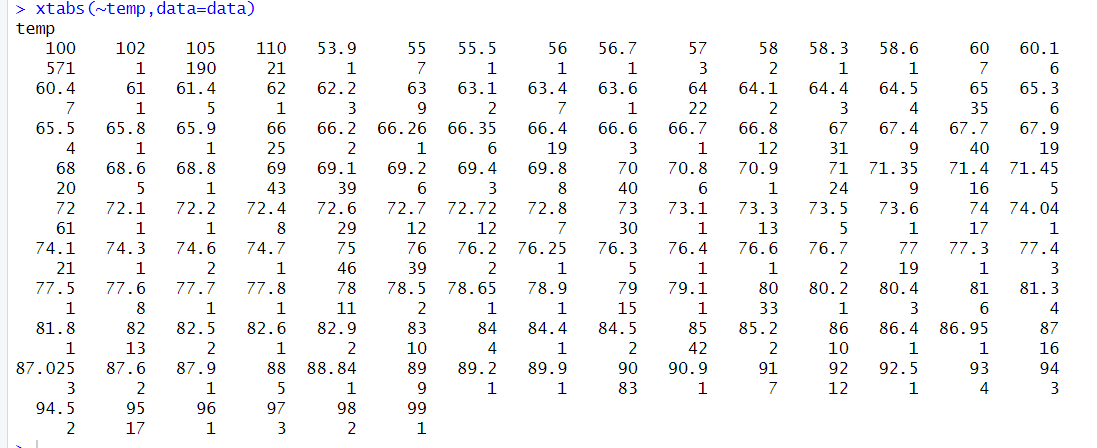
\includegraphics[width=\linewidth]{graphics/new_graphics/Xtabs/xtabs-temp.png}
        \caption{Summary of Temperature.}
    \end{subfigure}
    \caption{Summary of data by using command xtabs.}
\end{figure}
We remove the \mintinline{R}{NAs} rows from the data set, note that only the
\mintinline{R}{NAs} associated with specific columns are removed, the reason not to remove all is described in \textbf{Section \ref{subsection:data_cleaning}}.

\begin{code}{R}
    data <- data[!is.na(data$tdp), ]
    data <- data[!is.na(data$bfreq), ]
    data <- data[!is.na(data$litho), ]
    data <- data[!is.na(data$ncore), ]
    data <- data[!is.na(data$temp), ]
\end{code}

% END OF DATA CLEANING